\documentclass{article}
\usepackage[a4paper, top=3cm, bottom=3cm]{geometry}
\usepackage{setspace}
\usepackage{fancyhdr}
\usepackage{tocloft}
\usepackage[utf8x]{inputenc}
\usepackage[english]{babel}
\usepackage{url,graphicx,tabularx,array,geometry}
\usepackage{amsmath}
\usepackage{listings}
\usepackage{tikz}
\usepackage{listings}
\usepackage{courier}
\usepackage{caption}
\usepackage{titlesec}

\titleformat{\section}{\bf\Large\sffamily}{\thesection}{1em}{}  
\titleformat{\subsection}{\bf\large\large\sffamily}{\thesubsection}{1em}{}  

\lstset{
         basicstyle=\footnotesize\ttfamily, % Standardschrift
         %numbers=left,               % Ort der Zeilennummern
         numberstyle=\tiny,          % Stil der Zeilennummern
         %stepnumber=2,               % Abstand zwischen den Zeilennummern
         numbersep=5pt,              % Abstand der Nummern zum Text
         tabsize=2,                  % Groesse von Tabs
         extendedchars=true,         %
         breaklines=true,            % Zeilen werden Umgebrochen
         keywordstyle=\color{red},
    		frame=b,         
 %        keywordstyle=[1]\textbf,    % Stil der Keywords
 %        keywordstyle=[2]\textbf,    %
 %        keywordstyle=[3]\textbf,    %
 %        keywordstyle=[4]\textbf,   \sqrt{\sqrt{}} %
         stringstyle=\color{black}\ttfamily, % Farbe der String
         showspaces=false,           % Leerzeichen anzeigen ?
         showtabs=false,             % Tabs anzeigen ?
         xleftmargin=17pt,
         framexleftmargin=17pt,
         framexrightmargin=5pt,
         framexbottommargin=4pt,
         %backgroundcolor=\color{lightgray},
         showstringspaces=false      % Leerzeichen in Strings anzeigen ?        
 }
 \lstloadlanguages{% Check Dokumentation for further languages ...
         %[Visual]Basic
         %Pascal
         %C
         %C++
         %XML
         %HTML
         Java
 }

\DeclareCaptionFont{white}{\color{white}\sffamily}
\DeclareCaptionFormat{listing}{\colorbox[cmyk]{0.43, 0.35, 0.35,0.01}{\parbox{\textwidth}{\hspace{15pt}#1#2#3}}}
\captionsetup[lstlisting]{format=listing,labelfont=white,textfont=white, singlelinecheck=false, margin=0pt, font={bf,footnotesize}}

\def\ma{\textsc{Mason}}
\def\dm{\textsc{D-Mason}}

\begin{document}
\pagestyle{empty}
\sffamily
\title{\dm\: a tutorial}
\author{\url{http://www.isislab.it/projects/dmason}}
\maketitle

% Set arabic (1,2,3...) page numbering
\pagenumbering{arabic}


\section{Introduction}
We present a framework, \dm, that is a distributed version of  \ma, a well-known and popular library for writing and running Agent-based simulations. \dm\ introduces the parallelization at framework level so that scientists that use the framework (domain expert but with limited knowledge of distributed programming) can be only minimally aware of such distribution. 

In this document, in particular, we provide a step-by-step guide to the process of ``parallelization'' of the Particle example from \ma\ by using \dm.
\begin{figure}[ht]
	\centering
		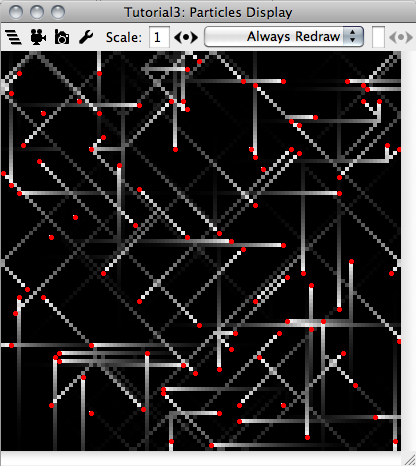
\includegraphics[width=0.5\textwidth, bb=0 0 470 520]{particles.png}	
		\caption{GUIState for \texttt{Particle} simulation}
	\label{fig:p01}
\end{figure}

\section{Acknowledgements}
\dm\ contains work by (in alphabetical order): \textit{Michele Carillo, Gennaro Cordasco, Rosario De Chiara, Fabio Fulgido, Ada Mancuso, Dario Mazzeo, Francesco Raia, Vittorio Scarano, Flavio Serrapica, Carmine Spagnuolo, 
Luca Vicidomini, Mario Fiore Vitale.}

\section{Structure}
The starting point is the package \texttt{Particles} is composed by three classes, as it can be found in the original MASON distribution:

\begin{itemize}
	\item \texttt{Particle:} it implements the agent that will be simulated by the application.
	\item \texttt{Particles:} it represents the simulation environment: it allows to run the simulation from the command line without using a GUI.
	\item \texttt{ParticlesWithUI:} it allows to run simulations with a GUI, as depicted in the Figure \ref{fig:p01}.
\end{itemize}

Similarly, in D-MASON, there will be the package \texttt{DParticles} containing the following classes:
\begin{itemize}
	\item \texttt{RemoteParticle:} it is an abstract class, implementing \texttt{RemoteAgent} and containing the remote ID of the agent in the field and its position. 
	\item \texttt{DParticle:} it extends \texttt{RemoteParticle} and implements the \texttt{distributed} agent that will be simulated by the application.
	\item \texttt{DParticles:} it represents the \texttt{distributed} simulation environment: it allows to run the simulation from the command line without using a GUI.
	\item \texttt{DParticlesWithUI:} it allows to run simulations with a GUI that is aware of the \texttt{distributed} environment.
\end{itemize}

\section{From \texttt{Particle} to \texttt{DParticle}}
The original \texttt{Particle} has to implement the \texttt{Steppable} interface and, in particular, the method \texttt{step()}, containing the agent logic. In the same way \texttt{RemoteParticle} is an abstract class that has to implement \texttt{RemoteAgent}, that is the D-MASON interface containing the necessary logic for the distributed agent. Finally \texttt{DParticle} extends \texttt{RemoteParticle} and implements the logic of the agent.

\texttt{RemoteAgent} is parameterized with an \texttt{Int2D} object-type because, in this simulation, the field has this specific type to indicate locations, and allows programmers to set, for each agent, an unique identifier and a field position.
A \texttt{Particle} simply contains two integer parameters, \texttt{xdir} and \texttt{ydir}, for setting the initial direction that the particle will move along.

\lstset{language=Java,caption={Class Particle},label=particle1}
\begin{lstlisting}
...
  public Particle(int xdir, int ydir) {
   public boolean randomize = false;
   this.xdir = xdir;
   this.ydir = ydir;
  }
...
\end{lstlisting}


\texttt{DParticle} has two constructors: the first is empty and it has been introduced for a future implementation of the method \texttt{clone()}, and the second one has as parameter a subclass of the abstract class \texttt{DistributedState}.

\lstset{language=Java,caption={Class DParticle},label=dparticle1}
\begin{lstlisting}
public class DParticle extends RemoteParticle<Int2D>
{
   public int xdir;  // -1, 0, or 1
   public int ydir;  // -1, 0, or 1

   public DParticle(){ }
   
   public DParticle(DistributedState state)
   {
     super(state);
   }
\end{lstlisting}

In order to distribute a MASON simulation it is necessary to change some parts of the agent logic. In the original MASON version each particle, on each step, performs a collision avoidance routine by checking whether the location it is moving to is already occupied by another particle or not. 

\lstset{language=Java,caption={Class Particle},label=particle2}
\begin{lstlisting}
   ...
  public void step(SimState state) {
   ...
   if (randomize) {
    xdir = tut.random.nextInt(3) - 1;
    ydir = tut.random.nextInt(3) - 1;
	  randomize = false;
   }
   ...
   // set my new location
   Int2D newloc = new Int2D(newx,newy);
   tut.particles.setObjectLocation(this,newloc);
   
   // randomize everyone at that location if need be
   Bag p = tut.particles.getObjectsAtLocation(newloc);
   if (p.numObjs > 1) {
   for(int x=0;x<p.numObjs;x++)
       ((Particle)(p.objs[x])).randomize = true;
   }
  }
}
\end{lstlisting}

The distributed version is slightly different because it first check if the new location is occupied and, in this case, it randomizes its direction and move to the new location by using the method \texttt{setDistributedObjectLocation}.

%In a distributed environment different particles cannot do this check in different steps, as in the original version, but they first check for collision, using the same MASON method, then they set the new field location, using \texttt{setDistributedObjectLocation}. 

\lstset{language=Java,caption={Class DParticle},label=dparticle2}
\begin{lstlisting}
public void step(SimState state)
{
 DParticles tut = (DParticles)state;
 Int2D location = tut.particles.getObjectLocation(this);
 Bag p = tut.particles.getObjectsAtLocation(location);
 tut.trails.setDistributedObjectLocation(1.0, location,state);
 if (p.numObjs > 1)
 {
   xdir = tut.random.nextInt(3) - 1; 
   ydir = tut.random.nextInt(3) - 1;
 }
 int newx = location.x + xdir;
 int newy = location.y + ydir;
 if (newx < 0) { newx++; xdir = -xdir; } 
 else if (newx >= tut.trails.getWidth()) {newx--; xdir = -xdir; }
 if (newy < 0) { newy++ ; ydir = -ydir; }
 else if (newy >= tut.trails.getHeight()) {newy--; ydir = -ydir; }
 Int2D newloc = new Int2D(newx,newy);
 tut.particles.setDistributedObjectLocation(newloc, this, state);
 }
}
\end{lstlisting}


\section{From \texttt{Particles} to \texttt{DParticles}}
\texttt{Particles} extends the \texttt{SimState} class  while \texttt{DParticles} extends \texttt{DistributedState}, parameterized with \texttt{Int2D} object-type.

DParticles contains three other variables indicating, respectively, width and height of the field and the way of partitioning the field (that can be one or two dimensional, as shown in Figure \ref{fig:dp01}). \texttt{Particles} has just one constructor that has as parameter the random generator seed while \texttt{DParticles} constructor has as input an objects array, containing several parameters specific for the distributed simulation (e.g. network address, port, etc \ldots). 

In \texttt{Particles} there are two fields, the first containing the agents, the second one containing the trails. The creation of the fields and the placement of the agents in them are carried out by a simple loop that instantiates new particles with a random position and direction and place them in the proper field. 

In order to add particles to the schedule, it is possible to use \texttt{scheduleRepeating()}, that allows to schedule agents repeatedly, and to add particles to the field there is \texttt{setObjectLocation()}. In \texttt{DParticles} there is the method \texttt{createDSparseGrid2D} of the class \texttt{DSparseGrid2DFactory} for creating a new distributed field. Note that it is necessary to use a factory to choose the kind of field partition. The agent initial position is computed by the method \texttt{setAvailableRandomLocation()} and to add particles in the schedule it is necessary to use the method \texttt{scheduleOnce()}, because in the next step a certain agent could not stay in the same part of the field, so using \texttt{scheduleRepeating()} will not delete the particle from the schedule. Finally there are other three new methods: a \texttt{getter} method for returning the subclass of the \texttt{DistributedState}, a method for adding an agent with a given position in the field, a method for attaching a portrayal to an agent.

\lstset{language=Java,caption={Class Particles},label=particles}
\begin{lstlisting}
public class Particles extends SimState  {
  public DoubleGrid2D trails;
  public SparseGrid2D particles;
  ...
  public Particles(long seed) {
      super(seed);
  }
  
  public void start() {
   ...
   for(int i=0 ; i<numParticles ; i++) {
     p = new Particle(random.nextInt(3) - 1, random.nextInt(3) - 1);  // random direction
     schedule.scheduleRepeating(p);
     ...
     particles.setObjectLocation(p,new Int2D(x,y));  // random location
   }
  }
  
  public static void main(String[] args) {
    doLoop(Particles.class, args);
    System.exit(0);
  }
}
\end{lstlisting}

\lstset{language=Java,caption={Class DParticles},label=dparticles}
\begin{lstlisting}
public class DParticles extends DistributedState<Int2D> {
private static boolean isToroidal=false;
public DSparseGrid2D particles;
public DDoubleGrid2D trails;
public int gridWidth ;
public int gridHeight ;
public int MODE;

public DParticles(Object[] params)
{
 super((Integer)params[2],(Integer)params[3],(Integer)params[4],
 (Integer)params[7], (Integer)params[8], (String)params[0],
 (String)params[1],(Integer)params[9], isToroidal,
 new DistributedMultiSchedule<Int2D>());
 ip = params[0]+"";
 port = params[1]+"";
 this.MODE=(Integer)params[9];
 gridWidth=(Integer)params[5];
 gridHeight=(Integer)params[6];
}

public void start()
{
 super.start();
 try
{
 trails = DDoubleGrid2DFactory.createDDoubleGrid2D(gridWidth,
  gridHeight, this, super.MAX_DISTANCE, TYPE.pos_i,
  TYPE.pos_j, super.NUMPEERS, MODE,0, false, "trails");

 particles = DSparseGrid2DFactory.createDSparseGrid2d(gridWidth,
  gridHeight, this, 
  super.MAX_DISTANCE, TYPE.pos_i,
  TYPE.pos_j,super.NUMPEERS,MODE, "particles");

 init_connection();
}catch (DMasonException e) { e.printStackTrace();}
 DParticle p=new DParticle(this);
 while(particles.size() != super.NUMAGENTS)
{
 particles.setAvailableRandomLocation(p);
 p.xdir = random.nextInt(3)-1;
 p.ydir = random.nextInt(3)-1;
 if(particles.setDistributedObjectLocationForPeer(new Int2D
   (p.pos.getX(),p.pos.getY()), p, this))
 {
 schedule.scheduleOnce(schedule.getTime()+1.0,p);
 if(particles.size() != super.NUMAGENTS)
 p=new DParticle(this);
 }
}
 Steppable decreaser = new Steppable()
{
 public void step(SimState state)
{
 trails.multiply(0.9);
}
 static final long serialVersionUID = 6330208160095250478L;
};
 schedule.scheduleRepeating(Schedule.EPOCH,2,decreaser,1);
try
{
 getTrigger().publishToTriggerTopic("Simulation cell "+particles.cellType+" ready...");
 } catch (Exception e) {
 e.printStackTrace();
 }
}

public static void main(String[] args)
{
 doLoop(DParticles.class, args);
 System.exit(0);
}
static final long serialVersionUID = 9115981605874680023L;

public DistributedField getField()
{
 return particles;
}

public SimState getState()
{
 return this;
}

public void addToField(RemoteAgent<Int2D> rm,Int2D loc)
{
 particles.setObjectLocation(rm, loc);
}

public boolean setPortrayalForObject(Object o)
 {
 return false;
 }
}

\end{lstlisting}

\section{From \texttt{ParticlesWithUI} to \texttt{DParticlesWithUI}}
\begin{figure}
\centering
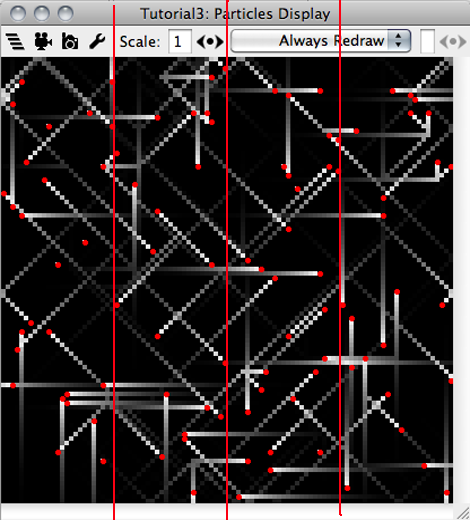
\includegraphics[width=0.4\textwidth,bb=0 0 470 520]{particles-h.png} 
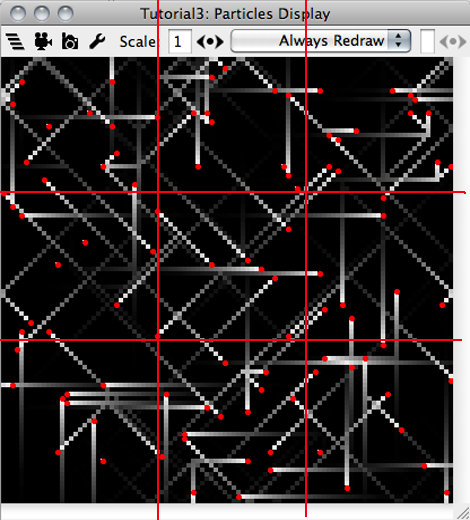
\includegraphics[width=0.4\textwidth,bb=0 0 470 520]{particles-m.png}
\caption{Respectively \texttt{HORIZONTAL} and \texttt{SQUARE} partition mode.}
\label{fig:dp01}
\end{figure}
There are few differences between original \texttt{ParticlesWithUI} and the its distributed version, \texttt{DParticlesWithUI}. They both extend the class \texttt{GUIState}, responsible of instantiating all graphics elements; \texttt{DParticlesWithUI} has a constructor for passing to \texttt{DParticles} the objects array and it has to store in a \texttt{String} the \texttt{region} identifier, in order to show which region it is simulating (e.g. \texttt{0-0} means the upper-left part of the grid partitioned field).
\lstset{language=Java,caption={Class ParticlesWithUI},label=particleswui}
\begin{lstlisting}
public class ParticlesWithUI extends GUIState {
...
public static void main(String[] args) {
ParticlesWithUI t = new ParticlesWithUI();
t.createController();
}
public ParticlesWithUI() { 
super(new Tutorial3(System.currentTimeMillis()));
}
public ParticlesWithUI(SimState state){
super(state);
}
...
}
\end{lstlisting}

\lstset{language=Java,caption={Class \texttt{DParticlesWithUI}},label=dparticleswui}
\begin{lstlisting}
public class DParticlesWithUI extends GUIState {
...
public static String name;
...
public DParticlesWithUI(Object[] args) {
super(new DParticles(args));
name = String.valueOf(
args[7])+""+(String.valueOf(args[8]));
}
public static String getName() { return "Peer: <"+name+">"; }
...
}
\end{lstlisting}

\section{Load balancing for Grid partition}

\section{Introduction}
As described before \dm\ uses a space partitioning approach where the fields are subdivided in regions assigned to workers; this approach allows to limit the communication among the workers. Indeed, since each agent interacts only within a small area around it, the communication is limited to local messages (messages between workers, managing neighboring spaces, etc.). 

The problem with this approach is that agents can migrate between regions and consequently the association between workers and agents changes during the simulation. Moreover, load balancing is not guaranteed and needs to be addressed by the application.

\subsection{The balancing mechanism}
The balancing mechanism is quite simple: when a region is overloaded it decides to split itself in smaller regions, dividing consequently the amount of agents in each of these regions. 

Two important factors have an impact on the efficiency of this decision: when to split and how to split.

Each region during the simulation compares the number $r$ of agents it is simulating with the average number $a$ of agents simulated by its neighbors. When these $r > k_s \times a$ then the load balancing kicks in splitting the overloaded region in $9$ subregions as depicted in \ref{fig:lb}: $8$ will go to neighbors of the overloaded region and it will be in charge just for the central one. 

As along as the inequality stands the region stays split; whenever $r < k_m \times a$ the subregions are called back to its original region. 

It is worth noting that the both the split and the merge are computational expensive operations so deciding the factors $k_s$ and $k_m$ is a key point in the performances of the whole system.

\begin{figure}[h!]
 \begin{center}
  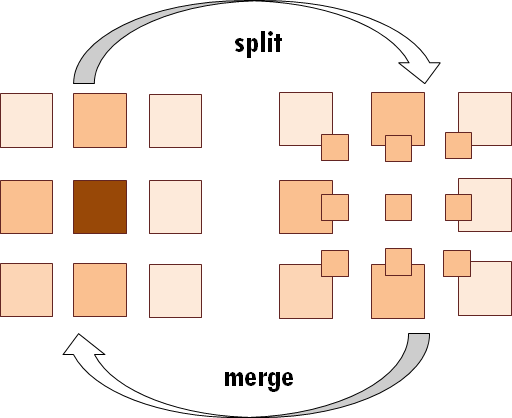
\includegraphics[width=0.5\textwidth, bb=0 0 512 418]{LoadBalancing.png}
  \caption{The load balance policy for split and merge: the darker region is overloaded and is split in $9$ subregions; when the load decreases the subregions are merged back. \label{fig:lb}}
 \end{center}
\end{figure}

\subsection{Parameters for load balancing}
In this section it is explained how to set the parameters for the load balancing in \texttt{DParticles}. The factor $k_s$ is the variable \texttt{thresholdSplit} and specifies while $k_m$ is the simulation parameter \texttt{thresholdMerge}.

\lstset{language=Java,caption={Class \texttt{DParticles}},label=dparticles2}
\begin{lstlisting}
 public DParticles(Object[] params)
    {    	
    	...
    	gridWidth = (Integer)params[5];
    	gridHeight = (Integer)params[6];
    	((DistributedMultiSchedule)schedule).setThresholdMerge(1);
        ((DistributedMultiSchedule)schedule).setThresholdSplit(5);

    }    
\end{lstlisting}

\subsection{Master GUI and load balancing}
To activate the load balancing mechanism the field must be square (same width and height) and its width (height) must be divisible by $3 \times sqrt(\#regions)$. For example when your field is divided in $16$ regions then the width (height) must be divisible by $3 \times \sqrt{16} = 12$. The number of regions must be $\geq9$ because of the way the split/merge mechanism works. The next step is just to tick the checkbox in Figure \ref{fig:masterlb}. 

\begin{figure}[ht!]
\centering {
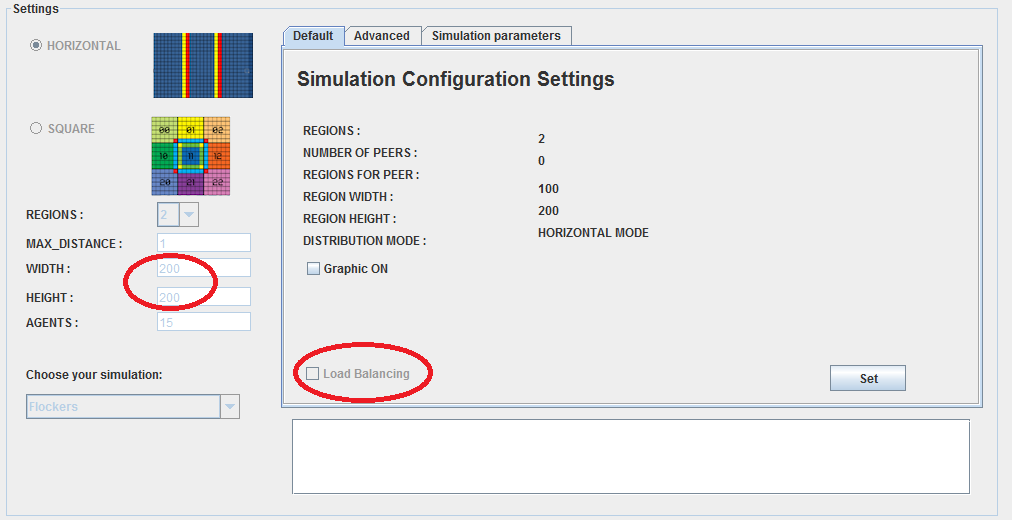
\includegraphics[width=0.9\textwidth, bb=0 0 1012 520]{JMasterUI.png}
\caption{Master GUI. \label{fig:masterlb}}}
\end{figure}

\section{System Management}

In this section it is explained the System Management functionalities, in detail:
\begin{description}
	\item[Peer Auto Reconnection] Automatic reconnection when the communication server (CS) is restarted after a failure;
	\item[Restart Simulation] Restart simulation without restart the CS (eg launch another simulation).
	\item[Jar Deploy] Deploy simulation/update jar to workers.
\end{description}

While the Peer Auto Reconnection is a mechanism that has been implemented at the framework level to enable the Simulation Reset requires to modify the ActiveMQ configuration file.

\paragraph*{Windows}
Under Windows the file to edit is \texttt{wrapper.conf} located in: 

\verb|%ACTIVEMQ_BASE%\bin\win32| or \verb|%ACTIVEMQ_BASE%\bin\win64|

In this file it is necessary to uncomment the following line:

\lstset{language=Java,caption={File \texttt{wrapper.conf}}}
\begin{lstlisting}
    	...
    	# Uncomment to enable jmx
	#wrapper.java.additional.n=-Dcom.sun.management.jmxremote.port = 1616
	#wrapper.java.additional.n=-Dcom.sun.management.jmxremote.authenticate = false
	#wrapper.java.additional.n=-Dcom.sun.management.jmxremote.ssl = false
\end{lstlisting}

and then replace the \texttt{n} with the next number from the previous section

\lstset{language=Java,caption={File \texttt{wrapper.conf}}}
\begin{lstlisting}
	...
	wrapper.java.additional.10 = -Dactivemq.conf = %ACTIVEMQ_CONF%
	wrapper.java.additional.11 = -Dactivemq.data = %ACTIVEMQ_DATA%
\end{lstlisting}

In this case we obtain this

\lstset{language=Java,caption={File \texttt{wrapper.conf}}}
\begin{lstlisting}
	...
	# Uncomment to enable remote jmx
	wrapper.java.additional.12=-Dcom.sun.management.jmxremote.port=1616
	wrapper.java.additional.13=-Dcom.sun.management.jmxremote.authenticate=false
	wrapper.java.additional.14=-Dcom.sun.management.jmxremote.ssl=false
\end{lstlisting}

\paragraph*{Linux}
Under Linux the file to edit is \textit{activemq} located in:

\verb|%ACTIVEMQ_HOME%/bin/|

It is necessary to uncomment this line

\lstset{language=Java,caption={File \texttt{activemq}},label=activemq}
\begin{lstlisting}
	...
	#
	#ACTIVEMQ_SUNJMX_START="-Dcom.sun.management.jmxremote.port=11099 "
	#ACTIVEMQ_SUNJMX_START="$ACTIVEMQ_SUNJMX_START -Dcom.sun.management.jmxremote.password.file=${ACTIVEMQ_CONF}/jmx.password"
	#ACTIVEMQ_SUNJMX_START="$ACTIVEMQ_SUNJMX_START -Dcom.sun.management.jmxremote.access.file=${ACTIVEMQ_CONF}/jmx.access"
	#ACTIVEMQ_SUNJMX_START="$ACTIVEMQ_SUNJMX_START -Dcom.sun.management.jmxremote.ssl=false"
	ACTIVEMQ_SUNJMX_START="$ACTIVEMQ_SUNJMX_START -Dcom.sun.management.jmxremote"
\end{lstlisting}

We obtain this
\lstset{language=Java,caption={File \texttt{activemq}},label=activemq2}
\begin{lstlisting}
	...
	#
	ACTIVEMQ_SUNJMX_START="-Dcom.sun.management.jmxremote.port=1616 "
	ACTIVEMQ_SUNJMX_START="$ACTIVEMQ_SUNJMX_START -Dcom.sun.management.jmxremote.authenticate=false"
	#ACTIVEMQ_SUNJMX_START="$ACTIVEMQ_SUNJMX_START -Dcom.sun.management.jmxremote.password.file=${ACTIVEMQ_CONF}/jmx.password"
	#ACTIVEMQ_SUNJMX_START="$ACTIVEMQ_SUNJMX_START -Dcom.sun.management.jmxremote.access.file=${ACTIVEMQ_CONF}/jmx.access"
	ACTIVEMQ_SUNJMX_START="$ACTIVEMQ_SUNJMX_START -Dcom.sun.management.jmxremote.ssl=false"
	#ACTIVEMQ_SUNJMX_START="$ACTIVEMQ_SUNJMX_START -Dcom.sun.management.jmxremote"

\end{lstlisting}
\subsection{How to use Master GUI to restart simulation}
To restart simulation there is reset button (in a the red circle in \ref{fig:mastersr}). When a simulation is stopped by clicking the button the parameters can be edit again and the simulation can be re-initialized.
\begin{figure}[h]
\centering{
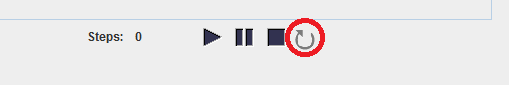
\includegraphics[scale= 0.5]{resetDetail.png}
\caption{Simulation reset button. \label{fig:mastersr}}}
\end{figure}

\subsection{Jar Deploy}
\subsubsection{Simulation Deploy}
This feature allows the user to quickly deploy a simulation on all the workers by using jar file.\\
\begin{figure}[h]
\centering{
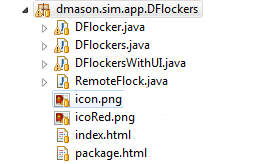
\includegraphics[scale=1]{images/simPackage.png}
\caption{An example: DFlockers simulation package. \label{fig:dflockpackage}}}
\end{figure}
Following we will describe the steps needed to generate a simulation jar file:
\begin{enumerate} 
  \item select the simulation package, right click on the package and choose export JAR file
  \item select the main class (i.e. DFlockers in our example)
\end{enumerate}

By using the  MasterUI (see Figure
\ref{fig:simjar})  application it is possible to deploy the created file to each worker and the Master.
\begin{figure}[h]
\centering{
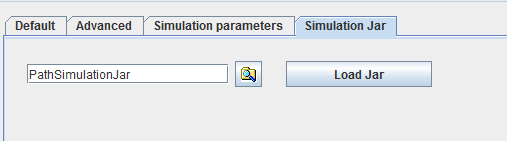
\includegraphics[scale=0.5]{images/simjar.png}
\caption{Simulation deploy in MasterUI. \label{fig:simjar}}}
\end{figure}\\
First of all the user has to choose the jar. Using the Simulation Jar tab the user can load the simulation jar file.
After this operation the simulation is available for the Master and can be chosen from the ``Choose your simulation'' combobox.
When a simulation is run by the Master, each worker will be able to download and run the corresponding simulation jar. 

\subsubsection{Worker update}
This feature allows the user to update the worker application.\\ 

Two different update methods have been provided:

\textbf{Manual Update.} The user can start a  manual update (which update all the active workers)  using the menu item System$\rightarrow$Update worker in the MasterUI application (see Figure \ref{fig:upmenu}). The update panel will appear (Figure \ref{fig:update}).
\begin{figure}[h!]
\centering{
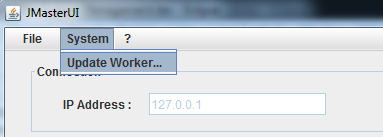
\includegraphics[scale=0.7]{images/updatemenu.png}
\caption{Manual update in MasterUI. \label{fig:upmenu}}}
\end{figure}
\begin{figure}[h]
\centering{
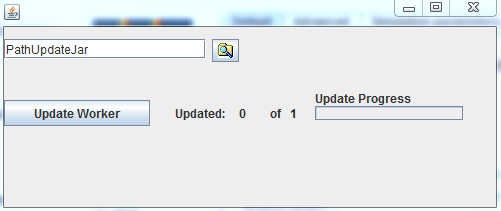
\includegraphics[scale=0.5]{images/update.png}
\caption{Manual update panel. \label{fig:update}}}
\end{figure}
In order to update the active workers, the user need to load the new application (a jar file). The update starts when the user   
clicks the ``Update Worker'' button. A progress bar will show the evolution of the update process.


\textbf{Automatic Update.} This procedure is still required since the manual update affects only active workers. Then when a new worker wake up it is important to check whether the workers need to be updated. The MasterUI is able to detect this problem (i.e. a worker not up to date) and automatically starts the update process.\\
The automatic update requires that the last worker jar file is available for the MasterUI application. When this file is not available a warning message appears in the MasterUI application (see Figure \ref{fig:mexfile}).
\begin{figure}[h]
\centering{
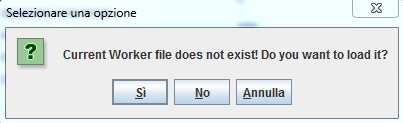
\includegraphics[scale=0.5]{images/mexfile.png}
\caption{Jar update not found. \label{fig:mexfile}}}
\end{figure}\\
When the MasterUI finds a worker which requires to be updated, a message will appear to inform that an updating process is going to start (see Figure \ref{fig:notsamever}).
\begin{figure}[h!]
\centering{
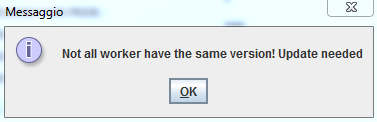
\includegraphics[scale=0.5]{images/notsamever.png}
\caption{Starting update process. \label{fig:notsamever}}}
\end{figure}

\newpage
\section{The Global Inspector}

Taking inspiration from the \ma inspector, we wanted to create a mechanism to let the user to inspect a distributed simulation. This is just a first a step toward a complete support of the mechanism.

\paragraph*{An example.}
Think about a simulation regarding inhabitants of a city. Suppose the simulation class exposes a method called \texttt{getPopulation()} returning an \texttt{int} representing the number of alive citizens.

Now assume that our city is split in a $2\times2$ grid. If any worker calls the \texttt{getPopulation()} on its region of the city, that call will return the number of alive citizen living in that region of the city. In this example, if we want to know how many citizens are alive in the entire city, we need to sum the number of citizens alive in each region.

This is the goal if the Global Inspector.

\subsection{Enabling the Global Inspector}
The Global Inspector (GI) is embedded into the Global Viewer. It allows the user to track specific statistics about the simulation being run, and also to view agent's positions.

In order to GI to work, we need build an \emph{inspectable} simulation, whose only goal will be to retrieve information from the workers, reduce it and show it in the model inspector.

Being the simulation class called \texttt{DParticles}, the GI will look for an inspectable class called  \texttt{DParticles\emph{Insp}}.

For each of the properties that the GI will display, the inspectable class will have:

\begin{itemize}
	\item a getter method (e.g. \texttt{getNumAgents()});  
  \item a reducer method (e.g. \texttt{reduceNumAgents()});
  \item possibly a variable (e.g. \texttt{numAgents})
\end{itemize}

This example may not have much sense, since the number of particles in this simulation never changes, but it is simple enough to get started. Following the details the class \texttt{DParticlesInsp}:

\lstset{language=Java,caption={Class DParticlesInsp},label=dparticlesinsp}
\begin{lstlisting}
public class DParticlesInsp extends InspectableState {
  protected int numAgents;

  public int getNumAgents() {
    return numAgents;
  }

  public void reduceNumAgents(Object[] shards) {
    int sum = 0;
    int n = shards.length;
    for (int i = 0; i < n; i++)
      sum += (Integer)shards[i];
    numAgents = sum;
  }
}
\end{lstlisting}

The reduce method takes an \texttt{Object[]} as parameter and the length of this array equals the number of regions in which the field is split and, obviously, each entry of the array contains information about one region (in no particular order).

A reduce method may have or not a return value. Remember that the global inspector reads the simulation status using getter methods so what the reduce method needs has to set a variable that will be read by the getter (in this case, \texttt{reduceNumAgents()}) set the variable \texttt{numAgents} that will be read by \texttt{getNumAgents()}.

\end{document}
